% Please use the skeleton file you have received in the
% invitation-to-submit email, where your data are already
% filled in. Otherwise please make sure you insert your
% data according to the instructions in PoSauthmanual.pdf
\documentclass{PoS}

\title{Concept Study for the Beamforming Elevated Array for Cosmic Neutrinos (BEACON)}

\ShortTitle{BEACON}

\author{\speaker{Stephanie Wissel}\thanks{A footnote may follow.}\\
        California Polytechnic State University\\
        E-mail: \email{swissel@calpoly.edu}}

%\author{Another Author\\
%        Affiliation\\
%        E-mail: \email{...}}

\abstract{Tau neutrinos are expected to comprise one third of both the astrophysical and cosmogenic neutrino flux, but currently the flavor ratio is poorly constrained and the expected flux at energies >100 PeV is low. We present a new concept for a radio detector called BEACON sensitive to tau neutrinos with energies greater than 100 PeV in which a radio interferometer searches for upgoing tau neutrinos from a high elevation mountain. Signals from several antennas are coherently summed at the trigger level, permitting not only directional masking of anthropogenic backgrounds, but also a lower trigger threshold. Simulation studies indicate that a modest array size and small number of stations can achieve competitive sensitivity, provided the receivers are at high enough elevation. As a proof of concept, an array of four 30-80 MHz dual polarized antennas was deployed at the White Mountain Research Station.}

\FullConference{36th International Cosmic Ray Conference -ICRC2019-\\
		July 24th - August 1st, 2019\\
		Madison, WI, U.S.A.}


\begin{document}
For oral and poster contributions, the maximum length of a paper is 8 pages including a title page and references.
\section{Motivation}
\begin{enumerate}
    \item 100 PeV extrapolated IceCube and GZK models predict comparable fluxes
    \item Different sources (unresolved IceCube sources vs. diffuse cosmic rays) predict transition in flavor ratios (right? check) as a function of energy
    \item Neutrino landscape in the 2020s:
        \begin{enumerate}
            \item IceCube, RNO, ANITA : sensitive to different regimes of the all-flavor neutrino flux
            \item Missing: ability to determine the tau fraction of the all-neutrino flux 
            \item Flavor ratios: source structure, p$\gamma$, pp interactions, composition (paper by Learned on different flavor ratios)
        \end{enumerate}
    \item BEACON : tau neutrino flux in the 100 PeV to 100 EeV regime
A low cost, fast option that can be deployed at multiple sites
    \begin{enumerate}
        \item Scalable
        \item Full-sky
        \item Logistically simple
        \item Mutli-messenger science drives need for 100\% duty cycle and full sky
        \item Follow-up on ANITA anomalous events
    \end{enumerate}
\end{enumerate}

To expand the reach of neutrino experiments into the PeV to EeV energy regime requires a dramatic improvement in acceptance and exposure at reasonable cost. We focus here on a concept that aims to maximize single station exposure to upgoing tau neutrinos using a phased interferometer on a high-elevation mountain. 

\section{Concept}
Lay out baseline concept : 120deg FOV, 3 km, acceptance from taus at horizon and nearby mountains

Several existing and proposed experiments search for the radio emission from  upgoing tau lepton decays resulting from tau neutrino interactions in the Earth\cite{Auger, GRAND, Trinity, POEMMA}. The BEACON concept differs in placing a phased interferometer on a high-elevation mountain. Mountain ridges of high prominence ($>2$~km), the difference between the elevation of the peaks and the viewable valley, maximize the individual station acceptance, while still being close enough to the air showers to maintain a low energy threshold. By phasing multiple antennas together in an interferometer, degree-scale pointing can be achieved and background events can be localized and removed from the trigger.

Upgoing tau neutrinos may be detected via the air showers that result from tau propagation and regneration through the Earth. Tau neutrinos are expected to interact in the Earth via charged current interactions that produce a tau lepton.% which decays with a decay length of $L_{decay} = XXX$ (function that depends on density in the rock) and with energy losses governed by the inelasticity and ... 
The tau lepton decay invariably results in another tau neutrino and this process can repeat until the particles reach the other side of the Earth. When this process results in a $\tau$ lepton exiting the Earth, the $\tau$ will decay within a decay length of $L_{decay} = 49 km (E_\tau/EeV)$ to produce an air shower. The probability that a tau will exit the Earth, $\P_{exit}$ depends on energy and emergence angle and is maximized for Earth skimming configurations with emergence angles $<3^{\circ}$ at energies greater than 0.1 EeV. 

Radio techniques are a promising method for the detection of ultra-high-energy particle air showers. The primary advantages are the low cost per channel of the instrumentation and the ability to trigger on showers from hundreds of kilometers away. Both are particularly important when considering the low expected flux of tau neutrinos at energies higher than 100 PeV and the geometric considerations associated with triggering on Earth skimming showers. Air showers produce broadband, impulsive signals at radio frequencies due to a combination of the geomagnetic and Askaryan effects. Cosmic rays experiments have successfully triggered on cosmic rays with radio-only triggers~\cite{TREND, OVRO-LWA} and recosntructed the air shower energies to within 14\%~\cite{AERA}.

\begin{figure}[htbp]
\begin{center}
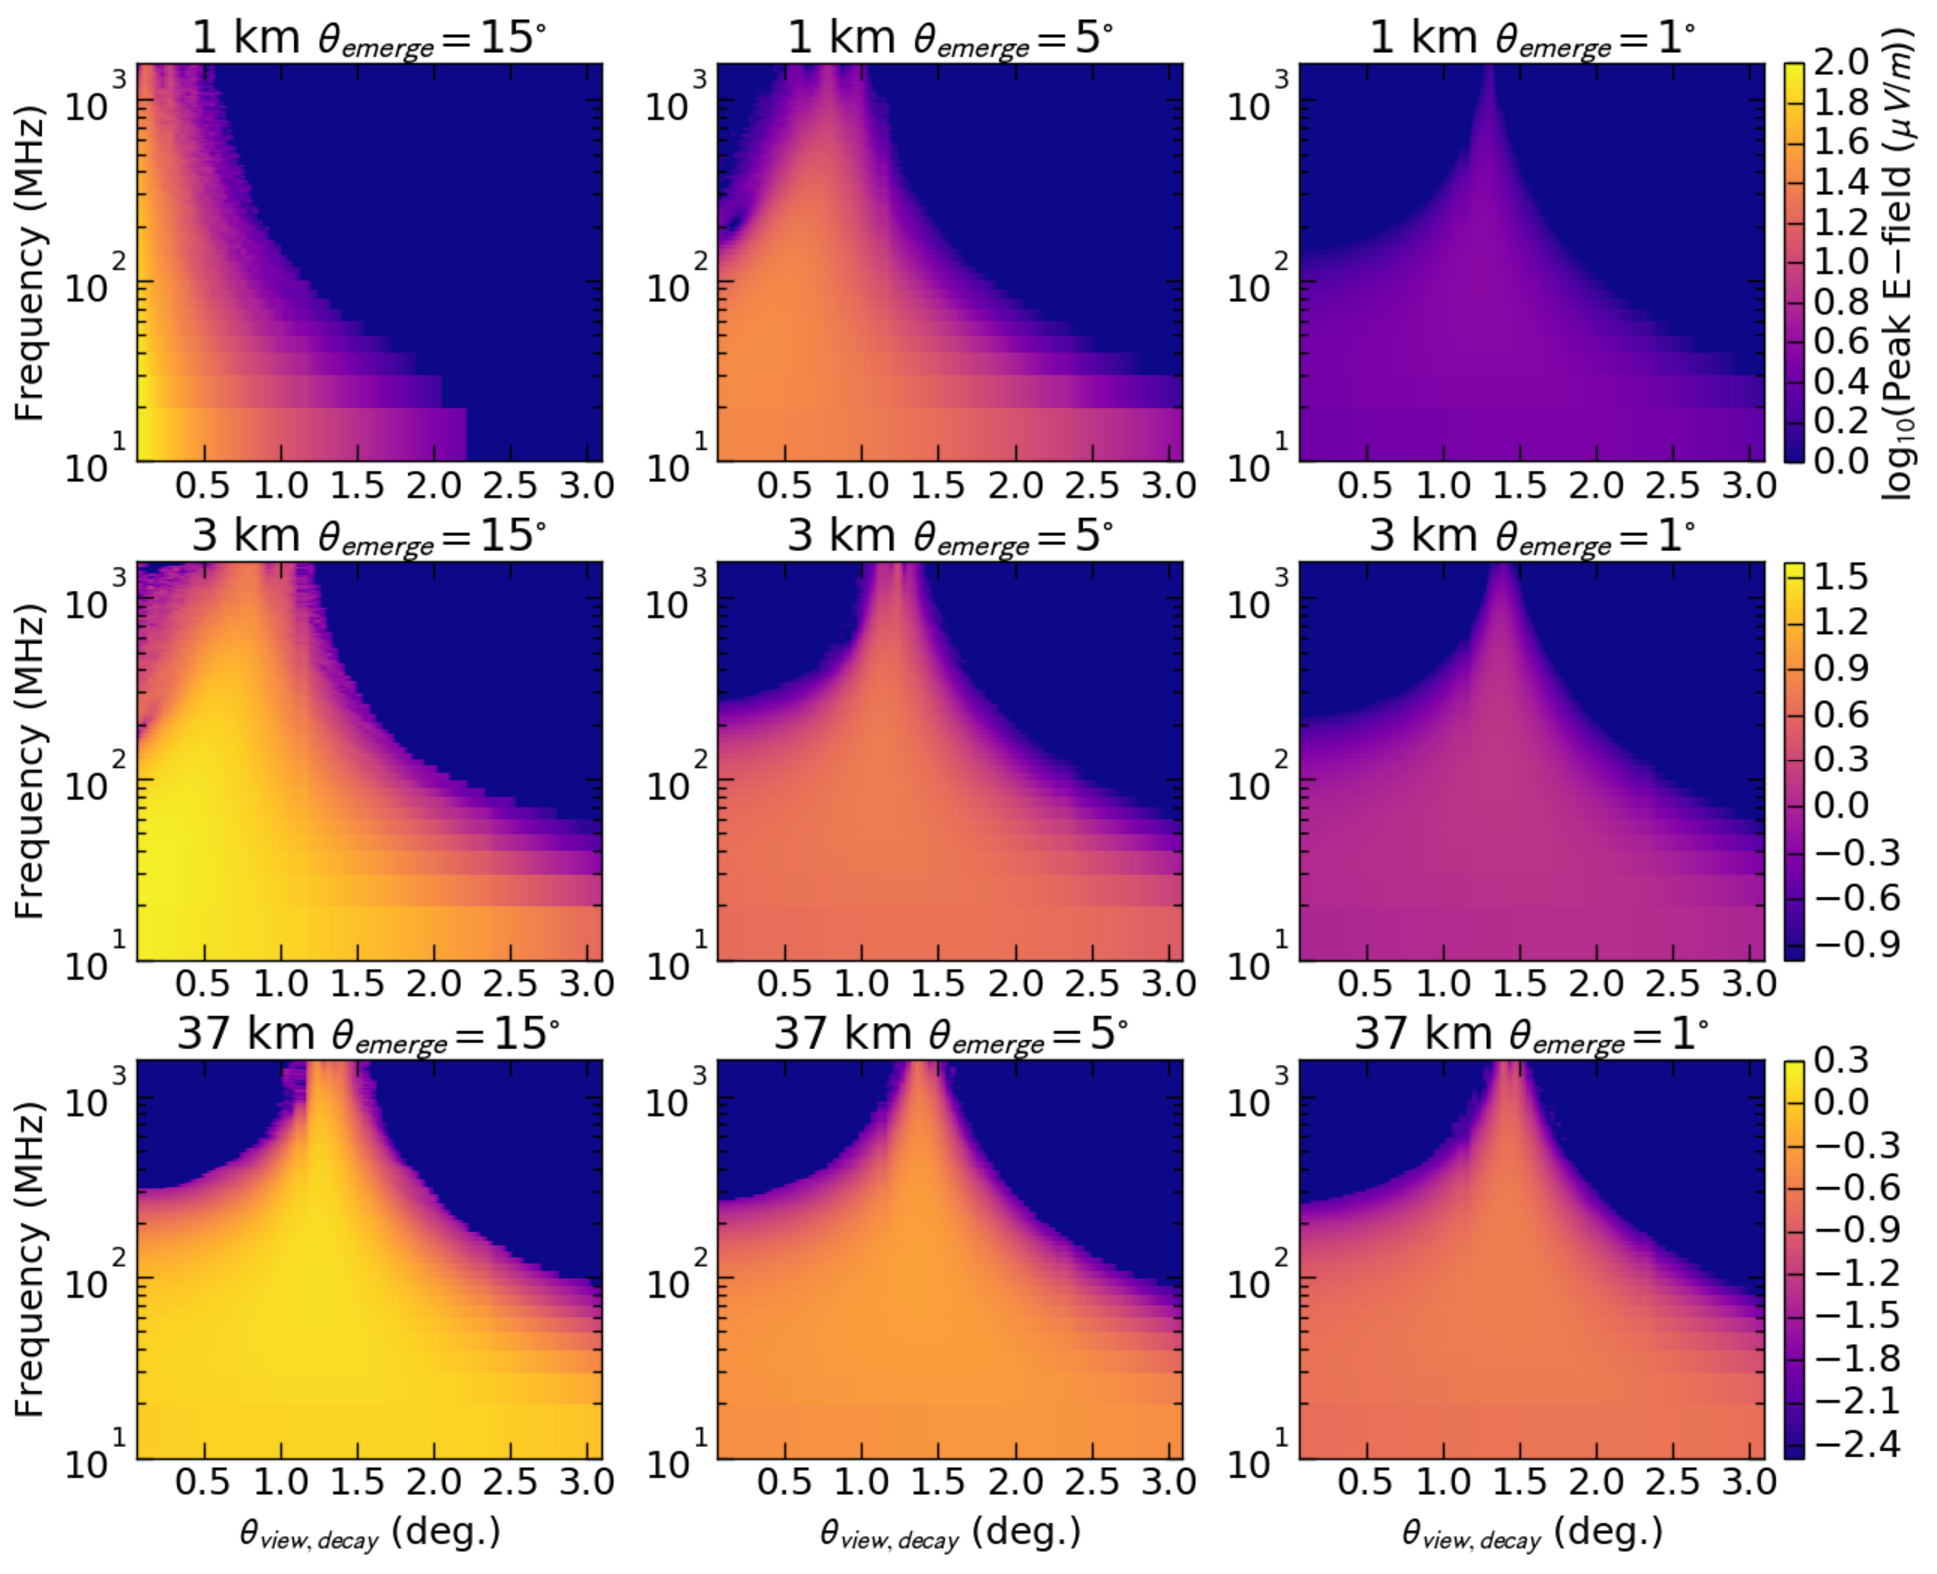
\includegraphics[width=\textwidth]{figures/efield_sims_logscale}
\caption{Peak electric field measured from ZHAireS simulations of upgoing tau lepton air showers.}
\label{fig:efield}
\end{center}
\end{figure}

Upgoing tau air showers are expected to generate broadband electric field signals such as those shown in Fig.~\ref{fig:efield}. Using ZHAireS modified for upgoing showers, we simulated showers measured at different elevations above sea level as measured by a line of antennas. The complete set of simulations included a range of tau emergence angles from 1$^{\circ}$ to 35$^{\circ}$, view angles $\theta_{view,decay}$ relative to the decay point of the shower (0-3.2$^{\circ}$), and tau lepton decay altitudes. Fig.~\ref{fig:efield} shows that the radio beam is broad at lower frequencies and forms a Cherenkov cone at highere frequencies. The Cherenkov cone notably does not form when the shower is too close to the detector at, for instance, high emergence angles and low detector altitudes. 

By sampling the radio signal in a broad range of frequencies, we can compare the performance of a high-elevation detector in different frequency bands. Integrating the peak electric field in a lower frequency band (30-80 MHz) and a higher frequency band (200-1200 MHz) yields the radio beams shown in Fig.~\ref{fig:SNR}. % add in how I calculate the thermal noise%
The lower frequency band has a broader radio beam since the region over which the radio emission is coherent is broader at longer wavelengths. However, the peak electric field measured in the higher frequency band is stronger at the Cherenkov angle both because the bandwidth is stronger and also because the expected thermal noise is weaker. The 30-80 MHz band is appropriate for strong signals originating from higher energy or more distant showers, while the higher frequency band may be better for detecting closer showers or lower energy showers.

\begin{figure}[htbp]
\begin{center}
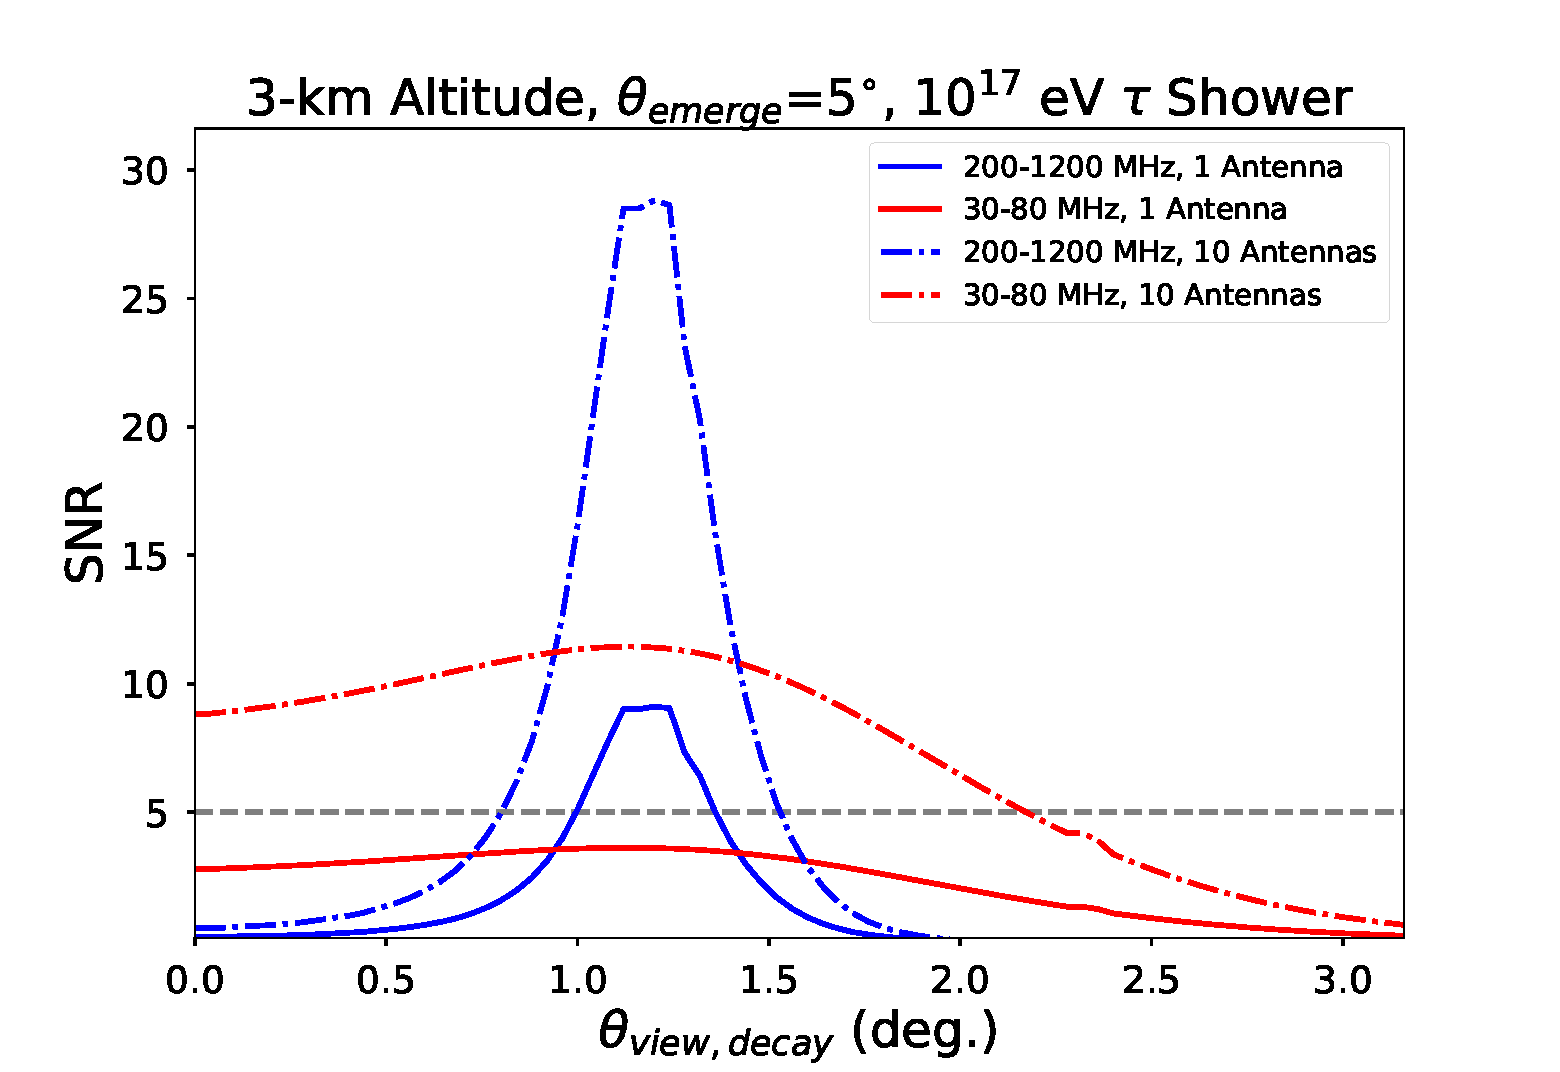
\includegraphics[width=\textwidth]{figures/SNR_example_emerge5deg_10antenna}
\caption{Signal-to-noise ratio}
\label{fig:SNR}
\end{center}
\end{figure}

Digital interferometric triggering in the time-domain has been shown to lower the voltage field threshold of an in-ice radio neutrino experiment~\cite{oberla_ara_pa} and to self-trigger on cosmic ray air showers using an array of 500 antennas~\cite{ryan_monroe}. When used in the context of BEACON, can take advantage of several features of phased array triggering to reduce anthropogenic backgrounds at the trigger level and lower the voltage and therefore energy threshold of the detector.

Consider an impulsive, band-limited, plane wave pulse arriving at a linear phased array at an angle $\theta$ with respect to the direction perpendicular to the array. The time delay $c \delta t$ between of the signal measured at an antenna at the center of the array measured at an antenna a distance $d$ from the center of the array is given by $c \delta t = d \sin \theta$. Beams in a particular direction can be formed knowing the precise geometry of the array by delaying and summing waveforms from multiple antennas in the time-domain. Digital phased arrays form beams on an FPGA via coherent sums of $N$ antennas at programmable angles. The signal-to-noise ratio of a neutrino radio pulse grows as a factor of $\sqrt{N}$, because the signal increases by a factor of $N$ while the incoherent thermal noise grows as $\sqrt{N}$. Since the electric field emitted by a given by fully formed air shower scales linearly with the energy, increasing the SNR of weaker signals lowers the energy threshold of the detector. 

\begin{enumerate}
    \item Interferometer 
    \item Directional rejection of background sources
    \item Man-made backgrounds are localized
    \item Coherent increase in SNR
    \item Pointing resolution limited by baseline length and radio beam width
    \item Large single station tau neutrino exposure
    \item High duty cycle
    \item Large FOV per station
    \item Sky Coverage
    \item Mid-latitude sites permit large sky coverage
    \item Multiple mountains to achieve full sky
    \item Tau neutrino flux
\end{enumerate}

\section{Results}

\subsection{10 Station Results}
\begin{enumerate}
    \item 10 antennas 
    \item Good angular resolution
    \item Improved sensitivity that traces the gain
    \item Beyond this, since stations independent, better to build more stations
    \item Differential acceptance  requires elevated antennas
    \item Point source sensitivity
    \item 10 station result
    \item Acceptance
    \item Minimum exposure required to do science
    \item Expected event rates
    \item Constraints on Kotera models, IceCube flux
\end{enumerate}

\subsection{100 Station Results}


The phased array technique presumes that the antennas are closely packed enough that each antenna in the array views a similar portion of the shower and is a similar distance from the showers. This suggests that the antennas should be closely packed with spacings set by several wavelengths of the detector.

When deciding on array layout, there is a tradeoff between the close packing desired for digital phasing and angular resolution. 


\begin{enumerate}
    \item 100 station result
    \item Acceptance
    \item Science you can do with 100 events
    \item IceCube 
    \item Complementarity with RNO
    \item Station separation
    \item Expected Energy resolution
    \item Expected Cosmic Ray rejection
\end{enumerate}

\begin{thebibliography}{99}
\bibitem{...}
....






\end{thebibliography}

\end{document}
